\documentclass{article}

\usepackage{noweb}
\noweboptions{smallcode,longchunks}
\usepackage[a4paper,margin=1in]{geometry}
\usepackage{colortbl}
\usepackage[colorlinks=true]{hyperref}
\usepackage{graphicx}

\newcommand{\hi}[1]{\noindent {\bf #1}}     % Define a handy paragraph opener

\def\nwendcode{\endtrivlist \endgroup}      % Remove noweb page break penalty
\let\nwdocspar=\par

\title{Jargo Simulation Controller\footnote{
  \url{https://github.com/jargors/Simulation-Controller}}}
\author{James J. Pan\\
  \small{\href{mailto:pan-j16@mails.tsinghua.edu.cn}{pan-j16@mails.tsinghua.edu.cn}}}

\begin{document}
\maketitle
\pagestyle{noweb}

\tableofcontents

\section{Introduction}
\label{sec:introduction}
The simulation controller is designed to be the sole means for an evaluation
program to control Jargo's simulation environment. The controller advances the
simulation world time, ``pushes'' server locations and new requests to the
client, perturbs server routes stored in the data layer in order to mimic
traffic and other stochastic vehicle processes, and can be used to report
evaluation metrics to the program. The controller sometimes needs to compute
shortest paths on the road network. It uses a compiled G-tree component to
compute paths quickly. The simulation controller is developed
using the Noweb\footnote{\url{https://www.cs.tufts.edu/~nr/noweb/}} literate
programming\footnote{\url{http://literateprogramming.com/}} tool.  This file
({\tt{}src/SimulationController.nw}) is the source for the documentation
({\tt{}doc/SimulationController.tex}) and the Java code
({\tt{}SimulationController.java})\footnote{See the {\tt{}Makefile} for build
details.}.

\begin{figure}[h]
\centering
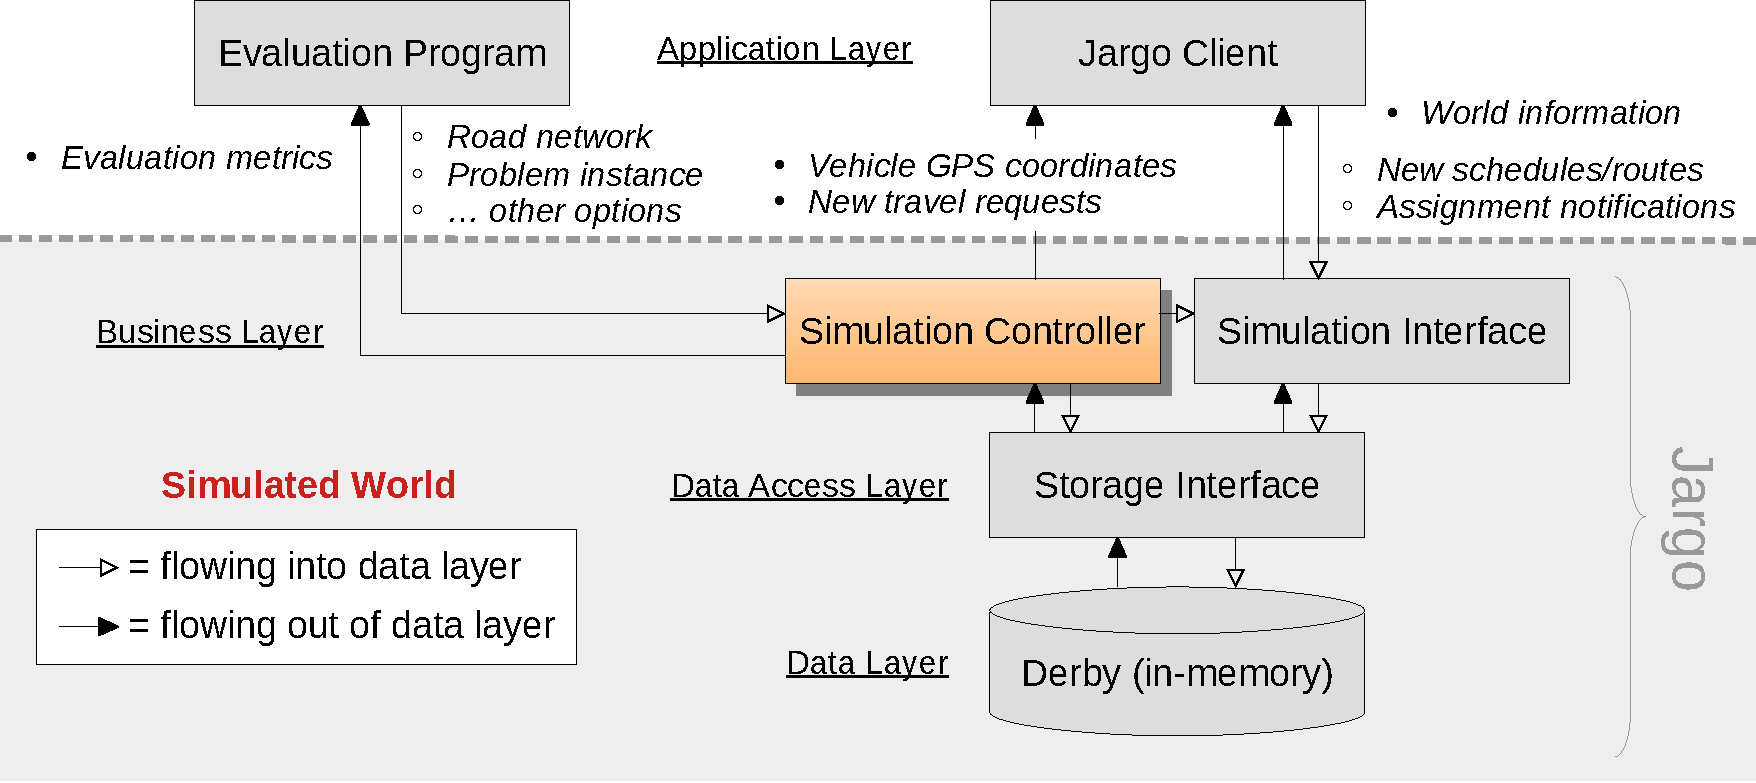
\includegraphics[width=150mm]{src/fig/controller-fig}
\caption{Controller within the Jargo stack.}
\label{fig:controller}
\end{figure}

\section{Implementation Overview}
The code consist of the \emph{preamble} (\S\ref{sec:preamble})
and the \emph{class definition} (\S\ref{sec:class-definition}).
\nwfilename{src/SimulationController.nw}\nwbegincode{1}\sublabel{NW3Xlx2m-wPE4K-1}\nwmargintag{{\nwtagstyle{}\subpageref{NW3Xlx2m-wPE4K-1}}}\moddef{SimulationController.java~{\nwtagstyle{}\subpageref{NW3Xlx2m-wPE4K-1}}}\endmoddef\nwnotused{SimulationController.java}
  \LA{}SimulationController.java preamble~{\nwtagstyle{}\subpageref{NW3Xlx2m-2MWOaE-1}}\RA{}
  \LA{}\code{}SimulationController\edoc{} definition~{\nwtagstyle{}\subpageref{NW3Xlx2m-2ZG2N7-1}}\RA{}
\nwendcode{}\nwbegindocs{2}\nwdocspar

\subsection{Preamble}
\label{sec:preamble}
The preamble declares the package and imports dependencies.
\nwenddocs{}\nwbegincode{3}\sublabel{NW3Xlx2m-2MWOaE-1}\nwmargintag{{\nwtagstyle{}\subpageref{NW3Xlx2m-2MWOaE-1}}}\moddef{SimulationController.java preamble~{\nwtagstyle{}\subpageref{NW3Xlx2m-2MWOaE-1}}}\endmoddef\nwalsodefined{\\{NW3Xlx2m-2MWOaE-2}\\{NW3Xlx2m-2MWOaE-3}\\{NW3Xlx2m-2MWOaE-4}\\{NW3Xlx2m-2MWOaE-5}\\{NW3Xlx2m-2MWOaE-6}}\nwused{\\{NW3Xlx2m-wPE4K-1}}
package com.github.jargors;
\nwendcode{}\nwbegindocs{4}\nwdocspar
We import:
\begin{itemize}
\item all parts of the Jargo stack;
\nwenddocs{}\nwbegincode{5}\sublabel{NW3Xlx2m-2MWOaE-2}\nwmargintag{{\nwtagstyle{}\subpageref{NW3Xlx2m-2MWOaE-2}}}\moddef{SimulationController.java preamble~{\nwtagstyle{}\subpageref{NW3Xlx2m-2MWOaE-1}}}\plusendmoddef
import com.github.jargors.StorageInterface;
import com.github.jargors.SimulationInterface;
import com.github.jargors.JargoClient;
import com.github.jargors.DistanceUtilities;
\nwendcode{}\nwbegindocs{6}\item standard utilities for concurrent execution;
\nwenddocs{}\nwbegincode{7}\sublabel{NW3Xlx2m-2MWOaE-3}\nwmargintag{{\nwtagstyle{}\subpageref{NW3Xlx2m-2MWOaE-3}}}\moddef{SimulationController.java preamble~{\nwtagstyle{}\subpageref{NW3Xlx2m-2MWOaE-1}}}\plusendmoddef
import java.util.concurrent.CompletableFuture;
import java.util.concurrent.Executors;
import java.util.concurrent.ScheduledExecutorService;
import java.util.concurrent.ScheduledFuture;
import java.util.concurrent.TimeUnit;
\nwendcode{}\nwbegindocs{8}\item various other utilities for file operations;
\nwenddocs{}\nwbegincode{9}\sublabel{NW3Xlx2m-2MWOaE-4}\nwmargintag{{\nwtagstyle{}\subpageref{NW3Xlx2m-2MWOaE-4}}}\moddef{SimulationController.java preamble~{\nwtagstyle{}\subpageref{NW3Xlx2m-2MWOaE-1}}}\plusendmoddef
import java.util.Scanner;
import java.io.File;
import java.io.FileNotFoundException;
\nwendcode{}\nwbegindocs{10}\item date-time class for printing timestamps;
\nwenddocs{}\nwbegincode{11}\sublabel{NW3Xlx2m-2MWOaE-5}\nwmargintag{{\nwtagstyle{}\subpageref{NW3Xlx2m-2MWOaE-5}}}\moddef{SimulationController.java preamble~{\nwtagstyle{}\subpageref{NW3Xlx2m-2MWOaE-1}}}\plusendmoddef
import java.time.LocalDateTime;
\nwendcode{}\nwbegindocs{12}\item standard map classes for caching user identifiers;
\nwenddocs{}\nwbegincode{13}\sublabel{NW3Xlx2m-2MWOaE-6}\nwmargintag{{\nwtagstyle{}\subpageref{NW3Xlx2m-2MWOaE-6}}}\moddef{SimulationController.java preamble~{\nwtagstyle{}\subpageref{NW3Xlx2m-2MWOaE-1}}}\plusendmoddef
import java.util.Map;
import java.util.HashMap;
\nwendcode{}\nwbegindocs{14}\nwdocspar
\end{itemize}

\subsection{Class Definition}
\label{sec:class-definition}
The {\tt{}SimulationController} class consists of member variables, a constructor,
and public and private methods, just like any other Java class. The controller
also comprises a static member function for loading the G-tree shared library.
\nwenddocs{}\nwbegincode{15}\sublabel{NW3Xlx2m-2ZG2N7-1}\nwmargintag{{\nwtagstyle{}\subpageref{NW3Xlx2m-2ZG2N7-1}}}\moddef{\code{}SimulationController\edoc{} definition~{\nwtagstyle{}\subpageref{NW3Xlx2m-2ZG2N7-1}}}\endmoddef\nwused{\\{NW3Xlx2m-wPE4K-1}}
public class SimulationController \{
  \LA{}\code{}SimulationController\edoc{} member variables~{\nwtagstyle{}\subpageref{NW3Xlx2m-15DcMp-1}}\RA{}
  \LA{}\code{}SimulationController\edoc{} constructor~{\nwtagstyle{}\subpageref{NW3Xlx2m-28Kazp-1}}\RA{}
  \LA{}\code{}SimulationController\edoc{} public methods~{\nwtagstyle{}\subpageref{NW3Xlx2m-45Q7Ei-1}}\RA{}
  \LA{}\code{}SimulationController\edoc{} private methods~{\nwtagstyle{}\subpageref{NW3Xlx2m-3kzkdD-1}}\RA{}
\}
\nwendcode{}\nwbegindocs{16}\nwdocspar

\subsection{Member Variables}
Member variables are grouped into \emph{containers}, \emph{settings}, and
\emph{loops}.
\nwenddocs{}\nwbegincode{17}\sublabel{NW3Xlx2m-15DcMp-1}\nwmargintag{{\nwtagstyle{}\subpageref{NW3Xlx2m-15DcMp-1}}}\moddef{\code{}SimulationController\edoc{} member variables~{\nwtagstyle{}\subpageref{NW3Xlx2m-15DcMp-1}}}\endmoddef\nwused{\\{NW3Xlx2m-2ZG2N7-1}}
\LA{}Container objects~{\nwtagstyle{}\subpageref{NW3Xlx2m-OUspt-1}}\RA{}
\LA{}Settings objects~{\nwtagstyle{}\subpageref{NW3Xlx2m-2svhLD-1}}\RA{}
\LA{}Loop objects~{\nwtagstyle{}\subpageref{NW3Xlx2m-2e0Sfa-1}}\RA{}
\nwendcode{}\nwbegindocs{18}\nwdocspar
\hi{Containers.}
\nwenddocs{}\nwbegincode{19}\sublabel{NW3Xlx2m-OUspt-1}\nwmargintag{{\nwtagstyle{}\subpageref{NW3Xlx2m-OUspt-1}}}\moddef{Container objects~{\nwtagstyle{}\subpageref{NW3Xlx2m-OUspt-1}}}\endmoddef\nwused{\\{NW3Xlx2m-15DcMp-1}}
private StorageInterface storage;
private SimulationInterface simulator;
private DistanceUtilities distance = new DistanceUtilities();
private JargoClient client;
private Map<Integer, Integer> userid = new HashMap<>();
private Map<Integer, int[]> lu_nodes = new HashMap<>();
\nwindexdefn{storage}{storage}{NW3Xlx2m-OUspt-1}\nwindexdefn{simulator}{simulator}{NW3Xlx2m-OUspt-1}\nwindexdefn{client}{client}{NW3Xlx2m-OUspt-1}\nwindexdefn{userid}{userid}{NW3Xlx2m-OUspt-1}\nwindexdefn{lu{\char95}nodes}{lu:unnodes}{NW3Xlx2m-OUspt-1}\eatline
\nwidentdefs{\\{{client}{client}}\\{{lu{\char95}nodes}{lu:unnodes}}\\{{simulator}{simulator}}\\{{storage}{storage}}\\{{userid}{userid}}}\nwendcode{}\nwbegindocs{20}\hi{Settings.} Settings objects configure various aspects of the simulation.
These settings should mostly be set by the evaluation program by using the public
setters.
\nwenddocs{}\nwbegincode{21}\sublabel{NW3Xlx2m-2svhLD-1}\nwmargintag{{\nwtagstyle{}\subpageref{NW3Xlx2m-2svhLD-1}}}\moddef{Settings objects~{\nwtagstyle{}\subpageref{NW3Xlx2m-2svhLD-1}}}\endmoddef\nwused{\\{NW3Xlx2m-15DcMp-1}}
private final double CSHIFT = 10000000.0;
private static int world_time = 0;
private int initial_world_time = 0;
private int final_world_time = 86400;
private int engine_update_period = 10;
private int loop_delay = 0;
\nwindexdefn{world{\char95}time}{world:untime}{NW3Xlx2m-2svhLD-1}\nwindexdefn{initial{\char95}world{\char95}time}{initial:unworld:untime}{NW3Xlx2m-2svhLD-1}\nwindexdefn{final{\char95}world{\char95}time}{final:unworld:untime}{NW3Xlx2m-2svhLD-1}\nwindexdefn{engine{\char95}update{\char95}period}{engine:unupdate:unperiod}{NW3Xlx2m-2svhLD-1}\nwindexdefn{loop{\char95}delay}{loop:undelay}{NW3Xlx2m-2svhLD-1}\eatline
\nwidentdefs{\\{{engine{\char95}update{\char95}period}{engine:unupdate:unperiod}}\\{{final{\char95}world{\char95}time}{final:unworld:untime}}\\{{initial{\char95}world{\char95}time}{initial:unworld:untime}}\\{{loop{\char95}delay}{loop:undelay}}\\{{world{\char95}time}{world:untime}}}\nwendcode{}\nwbegindocs{22}\hi{Loops.} Jargo's simulation environment comprises four ``loops'', defined
here, running in parallel. They are executed using Java's
{\tt{}ScheduledExecutorService} to control timing.
\nwenddocs{}\nwbegincode{23}\sublabel{NW3Xlx2m-2e0Sfa-1}\nwmargintag{{\nwtagstyle{}\subpageref{NW3Xlx2m-2e0Sfa-1}}}\moddef{Loop objects~{\nwtagstyle{}\subpageref{NW3Xlx2m-2e0Sfa-1}}}\endmoddef\nwused{\\{NW3Xlx2m-15DcMp-1}}
\LA{}Definition of clock loop~{\nwtagstyle{}\subpageref{NW3Xlx2m-2lFPcZ-1}}\RA{}
\LA{}Definition of engine loop~{\nwtagstyle{}\subpageref{NW3Xlx2m-3rcRXt-1}}\RA{}
\LA{}Definition of request collection loop~{\nwtagstyle{}\subpageref{NW3Xlx2m-10L3rI-1}}\RA{}
\LA{}Definition of server collection loop~{\nwtagstyle{}\subpageref{NW3Xlx2m-1I3SnY-1}}\RA{}
\nwendcode{}\nwbegindocs{24}\nwdocspar

\subsubsection{Clock Loop}
This loop advances the simulation world time.
\nwenddocs{}\nwbegincode{25}\sublabel{NW3Xlx2m-2lFPcZ-1}\nwmargintag{{\nwtagstyle{}\subpageref{NW3Xlx2m-2lFPcZ-1}}}\moddef{Definition of clock loop~{\nwtagstyle{}\subpageref{NW3Xlx2m-2lFPcZ-1}}}\endmoddef\nwused{\\{NW3Xlx2m-2e0Sfa-1}}
private Runnable ClockLoop = new Runnable() \{
  public void run() \{
    world_time++;
    simulator.setSimulationWorldTime(world_time);
    storage.printSQLDriverStatistics();
  \}
\};
\nwindexdefn{ClockLoop}{ClockLoop}{NW3Xlx2m-2lFPcZ-1}\eatline
\nwidentdefs{\\{{ClockLoop}{ClockLoop}}}\nwidentuses{\\{{simulator}{simulator}}\\{{storage}{storage}}\\{{world{\char95}time}{world:untime}}}\nwindexuse{simulator}{simulator}{NW3Xlx2m-2lFPcZ-1}\nwindexuse{storage}{storage}{NW3Xlx2m-2lFPcZ-1}\nwindexuse{world{\char95}time}{world:untime}{NW3Xlx2m-2lFPcZ-1}\nwendcode{}\nwbegindocs{26}\nwdocspar
\subsubsection{Engine Loop}
TODO: Stochastic processes (e.g. traffic) will go here.
\nwenddocs{}\nwbegincode{27}\sublabel{NW3Xlx2m-3rcRXt-1}\nwmargintag{{\nwtagstyle{}\subpageref{NW3Xlx2m-3rcRXt-1}}}\moddef{Definition of engine loop~{\nwtagstyle{}\subpageref{NW3Xlx2m-3rcRXt-1}}}\endmoddef\nwused{\\{NW3Xlx2m-2e0Sfa-1}}
private Runnable EngineLoop = new Runnable() \{
  public void run() \{
    // Print("I am EngineLoop running on "+Thread.currentThread().getName());
  \}
\};
\nwindexdefn{EngineLoop}{EngineLoop}{NW3Xlx2m-3rcRXt-1}\eatline
\nwidentdefs{\\{{EngineLoop}{EngineLoop}}}\nwidentuses{\\{{Print}{Print}}}\nwindexuse{Print}{Print}{NW3Xlx2m-3rcRXt-1}\nwendcode{}\nwbegindocs{28}\nwdocspar
\subsubsection{Request Loop}
This loop ``pushes'' queued requests to the client.
\nwenddocs{}\nwbegincode{29}\sublabel{NW3Xlx2m-10L3rI-1}\nwmargintag{{\nwtagstyle{}\subpageref{NW3Xlx2m-10L3rI-1}}}\moddef{Definition of request collection loop~{\nwtagstyle{}\subpageref{NW3Xlx2m-10L3rI-1}}}\endmoddef\nwused{\\{NW3Xlx2m-2e0Sfa-1}}
private Runnable RequestLoop = () -> \{
  final int t0 = world_time;
  int[] output = storage.DBQueryQueuedRequests(world_time);
  final int t1 = world_time;
  Print("RequestLoop t0="+t0+", t1="+t1+", # of requests="+output.length/7);
  client.collectRequests(output);
\};
\nwindexdefn{RequestLoop}{RequestLoop}{NW3Xlx2m-10L3rI-1}\eatline
\nwidentdefs{\\{{RequestLoop}{RequestLoop}}}\nwidentuses{\\{{client}{client}}\\{{Print}{Print}}\\{{storage}{storage}}\\{{world{\char95}time}{world:untime}}}\nwindexuse{client}{client}{NW3Xlx2m-10L3rI-1}\nwindexuse{Print}{Print}{NW3Xlx2m-10L3rI-1}\nwindexuse{storage}{storage}{NW3Xlx2m-10L3rI-1}\nwindexuse{world{\char95}time}{world:untime}{NW3Xlx2m-10L3rI-1}\nwendcode{}\nwbegindocs{30}\nwdocspar
\subsubsection{Server Loop}
This loop ``pushes'' server locations to the client.
\nwenddocs{}\nwbegincode{31}\sublabel{NW3Xlx2m-1I3SnY-1}\nwmargintag{{\nwtagstyle{}\subpageref{NW3Xlx2m-1I3SnY-1}}}\moddef{Definition of server collection loop~{\nwtagstyle{}\subpageref{NW3Xlx2m-1I3SnY-1}}}\endmoddef\nwused{\\{NW3Xlx2m-2e0Sfa-1}}
private Runnable ServerLoop = () -> \{
  final int t0 = world_time;
  int[] output = storage.DBQueryServerLocationsActive(world_time);
  final int t1 = world_time;
  Print("ServerLoop t0="+t0+", t1="+t1+", # of servers="+output.length/3);
  client.collectServerLocations(output);
\};
\nwindexdefn{ServerLoop}{ServerLoop}{NW3Xlx2m-1I3SnY-1}\eatline
\nwidentdefs{\\{{ServerLoop}{ServerLoop}}}\nwidentuses{\\{{client}{client}}\\{{Print}{Print}}\\{{storage}{storage}}\\{{world{\char95}time}{world:untime}}}\nwindexuse{client}{client}{NW3Xlx2m-1I3SnY-1}\nwindexuse{Print}{Print}{NW3Xlx2m-1I3SnY-1}\nwindexuse{storage}{storage}{NW3Xlx2m-1I3SnY-1}\nwindexuse{world{\char95}time}{world:untime}{NW3Xlx2m-1I3SnY-1}\nwendcode{}\nwbegindocs{32}\nwdocspar
\subsection{Constructor}
\nwenddocs{}\nwbegincode{33}\sublabel{NW3Xlx2m-28Kazp-1}\nwmargintag{{\nwtagstyle{}\subpageref{NW3Xlx2m-28Kazp-1}}}\moddef{\code{}SimulationController\edoc{} constructor~{\nwtagstyle{}\subpageref{NW3Xlx2m-28Kazp-1}}}\endmoddef\nwused{\\{NW3Xlx2m-2ZG2N7-1}}
public SimulationController() \{
  this.storage = new StorageInterface();
  this.simulator = new SimulationInterface(storage);
\}
\nwidentuses{\\{{simulator}{simulator}}\\{{storage}{storage}}}\nwindexuse{simulator}{simulator}{NW3Xlx2m-28Kazp-1}\nwindexuse{storage}{storage}{NW3Xlx2m-28Kazp-1}\nwendcode{}\nwbegindocs{34}\nwdocspar

\section{Public Methods}
\label{sec:public-methods}
\hi{General methods.}
\nwenddocs{}\nwbegincode{35}\sublabel{NW3Xlx2m-45Q7Ei-1}\nwmargintag{{\nwtagstyle{}\subpageref{NW3Xlx2m-45Q7Ei-1}}}\moddef{\code{}SimulationController\edoc{} public methods~{\nwtagstyle{}\subpageref{NW3Xlx2m-45Q7Ei-1}}}\endmoddef\nwalsodefined{\\{NW3Xlx2m-45Q7Ei-2}}\nwused{\\{NW3Xlx2m-2ZG2N7-1}}
\LA{}Set client~{\nwtagstyle{}\subpageref{NW3Xlx2m-3HnCZ3-1}}\RA{}
\LA{}Set initial world time~{\nwtagstyle{}\subpageref{NW3Xlx2m-3BZAWj-1}}\RA{}
\LA{}Set final world time~{\nwtagstyle{}\subpageref{NW3Xlx2m-2PAB4K-1}}\RA{}
\LA{}Get world time~{\nwtagstyle{}\subpageref{NW3Xlx2m-3X8zhz-1}}\RA{}
\LA{}Save backup~{\nwtagstyle{}\subpageref{NW3Xlx2m-2OKmqF-1}}\RA{}
\LA{}Load backup~{\nwtagstyle{}\subpageref{NW3Xlx2m-b3Hn1-1}}\RA{}
\LA{}Load data model~{\nwtagstyle{}\subpageref{NW3Xlx2m-4P4YpK-1}}\RA{}
\LA{}Load road network~{\nwtagstyle{}\subpageref{NW3Xlx2m-1JUvcB-1}}\RA{}
\LA{}Load problem~{\nwtagstyle{}\subpageref{NW3Xlx2m-2rtVpi-1}}\RA{}
\LA{}Load GTree~{\nwtagstyle{}\subpageref{NW3Xlx2m-b7Jka-1}}\RA{}
\LA{}Start simulation~{\nwtagstyle{}\subpageref{NW3Xlx2m-1DbeL0-1}}\RA{}
\nwendcode{}\nwbegindocs{36}\nwdocspar
\hi{Read methods.}
\nwenddocs{}\nwbegincode{37}\sublabel{NW3Xlx2m-45Q7Ei-2}\nwmargintag{{\nwtagstyle{}\subpageref{NW3Xlx2m-45Q7Ei-2}}}\moddef{\code{}SimulationController\edoc{} public methods~{\nwtagstyle{}\subpageref{NW3Xlx2m-45Q7Ei-1}}}\plusendmoddef
\LA{}Query custom statement~{\nwtagstyle{}\subpageref{NW3Xlx2m-2FtqIZ-1}}\RA{}
\LA{}Query ridesharing user~{\nwtagstyle{}\subpageref{NW3Xlx2m-3isdeu-1}}\RA{}
\LA{}Query routes~{\nwtagstyle{}\subpageref{NW3Xlx2m-1AprqI-1}}\RA{}
\LA{}Query schedules~{\nwtagstyle{}\subpageref{NW3Xlx2m-3yA8FQ-1}}\RA{}
\LA{}Query various metrics~{\nwtagstyle{}\subpageref{NW3Xlx2m-1Ang64-1}}\RA{}
\nwendcode{}\nwbegindocs{38}\nwdocspar

\subsection{General methods}

\subsubsection{{\tt{}\protect\nosublabel{NW3Xlx2m-45Q7Ei-2-u5}\protect\nwindexuse{setClient}{setClient}{NW3Xlx2m-3HnCZ3-1}setClient}(1)}
\nwenddocs{}\nwbegincode{39}\sublabel{NW3Xlx2m-3HnCZ3-1}\nwmargintag{{\nwtagstyle{}\subpageref{NW3Xlx2m-3HnCZ3-1}}}\moddef{Set client~{\nwtagstyle{}\subpageref{NW3Xlx2m-3HnCZ3-1}}}\endmoddef\nwused{\\{NW3Xlx2m-45Q7Ei-1}}
public void setClient(JargoClient target) \{
  client = target;
\}
\nwindexdefn{setClient}{setClient}{NW3Xlx2m-3HnCZ3-1}\eatline
\nwidentdefs{\\{{setClient}{setClient}}}\nwidentuses{\\{{client}{client}}}\nwindexuse{client}{client}{NW3Xlx2m-3HnCZ3-1}\nwendcode{}\nwbegindocs{40}\nwdocspar
\subsubsection{{\tt{}\protect\nwindexuse{setInitialWorldTime}{setInitialWorldTime}{NW3Xlx2m-3BZAWj-1}setInitialWorldTime(1)}}
\nwenddocs{}\nwbegincode{41}\sublabel{NW3Xlx2m-3BZAWj-1}\nwmargintag{{\nwtagstyle{}\subpageref{NW3Xlx2m-3BZAWj-1}}}\moddef{Set initial world time~{\nwtagstyle{}\subpageref{NW3Xlx2m-3BZAWj-1}}}\endmoddef\nwused{\\{NW3Xlx2m-45Q7Ei-1}}
public void setInitialWorldTime(int t) \{
  initial_world_time = t;
\}
\nwindexdefn{setInitialWorldTime}{setInitialWorldTime}{NW3Xlx2m-3BZAWj-1}\eatline
\nwidentdefs{\\{{setInitialWorldTime}{setInitialWorldTime}}}\nwidentuses{\\{{initial{\char95}world{\char95}time}{initial:unworld:untime}}}\nwindexuse{initial{\char95}world{\char95}time}{initial:unworld:untime}{NW3Xlx2m-3BZAWj-1}\nwendcode{}\nwbegindocs{42}\nwdocspar
\subsubsection{{\tt{}\protect\nwindexuse{setFinalWorldTime}{setFinalWorldTime}{NW3Xlx2m-2PAB4K-1}setFinalWorldTime(1)}}
\nwenddocs{}\nwbegincode{43}\sublabel{NW3Xlx2m-2PAB4K-1}\nwmargintag{{\nwtagstyle{}\subpageref{NW3Xlx2m-2PAB4K-1}}}\moddef{Set final world time~{\nwtagstyle{}\subpageref{NW3Xlx2m-2PAB4K-1}}}\endmoddef\nwused{\\{NW3Xlx2m-45Q7Ei-1}}
public void setFinalWorldTime(int t) \{
  final_world_time = t;
\}
\nwindexdefn{setFinalWorldTime}{setFinalWorldTime}{NW3Xlx2m-2PAB4K-1}\eatline
\nwidentdefs{\\{{setFinalWorldTime}{setFinalWorldTime}}}\nwidentuses{\\{{final{\char95}world{\char95}time}{final:unworld:untime}}}\nwindexuse{final{\char95}world{\char95}time}{final:unworld:untime}{NW3Xlx2m-2PAB4K-1}\nwendcode{}\nwbegindocs{44}\nwdocspar
\subsubsection{{\tt{}\protect\nwindexuse{getSimulationWorldTime}{getSimulationWorldTime}{NW3Xlx2m-3X8zhz-1}getSimulationWorldTime(0)}}
\nwenddocs{}\nwbegincode{45}\sublabel{NW3Xlx2m-3X8zhz-1}\nwmargintag{{\nwtagstyle{}\subpageref{NW3Xlx2m-3X8zhz-1}}}\moddef{Get world time~{\nwtagstyle{}\subpageref{NW3Xlx2m-3X8zhz-1}}}\endmoddef\nwused{\\{NW3Xlx2m-45Q7Ei-1}}
public static int getSimulationWorldTime() \{
  return world_time;
\}
\nwindexdefn{getSimulationWorldTime}{getSimulationWorldTime}{NW3Xlx2m-3X8zhz-1}\eatline
\nwidentdefs{\\{{getSimulationWorldTime}{getSimulationWorldTime}}}\nwidentuses{\\{{world{\char95}time}{world:untime}}}\nwindexuse{world{\char95}time}{world:untime}{NW3Xlx2m-3X8zhz-1}\nwendcode{}\nwbegindocs{46}\nwdocspar
\subsubsection{{\tt{}save}(1)}
\nwenddocs{}\nwbegincode{47}\sublabel{NW3Xlx2m-2OKmqF-1}\nwmargintag{{\nwtagstyle{}\subpageref{NW3Xlx2m-2OKmqF-1}}}\moddef{Save backup~{\nwtagstyle{}\subpageref{NW3Xlx2m-2OKmqF-1}}}\endmoddef\nwused{\\{NW3Xlx2m-45Q7Ei-1}}
public void saveBackup(String p) \{
  storage.DBSaveBackup(p);
\}
\nwindexdefn{saveBackup}{saveBackup}{NW3Xlx2m-2OKmqF-1}\eatline
\nwidentdefs{\\{{saveBackup}{saveBackup}}}\nwidentuses{\\{{storage}{storage}}}\nwindexuse{storage}{storage}{NW3Xlx2m-2OKmqF-1}\nwendcode{}\nwbegindocs{48}\nwdocspar
\subsubsection{{\tt{}\protect\nwindexuse{loadBackup}{loadBackup}{NW3Xlx2m-b3Hn1-1}loadBackup}(1)}
\nwenddocs{}\nwbegincode{49}\sublabel{NW3Xlx2m-b3Hn1-1}\nwmargintag{{\nwtagstyle{}\subpageref{NW3Xlx2m-b3Hn1-1}}}\moddef{Load backup~{\nwtagstyle{}\subpageref{NW3Xlx2m-b3Hn1-1}}}\endmoddef\nwused{\\{NW3Xlx2m-45Q7Ei-1}}
public void loadBackup(String p) \{
  storage.DBLoadBackup(p);
\}
\nwindexdefn{loadBackup}{loadBackup}{NW3Xlx2m-b3Hn1-1}\eatline
\nwidentdefs{\\{{loadBackup}{loadBackup}}}\nwidentuses{\\{{storage}{storage}}}\nwindexuse{storage}{storage}{NW3Xlx2m-b3Hn1-1}\nwendcode{}\nwbegindocs{50}\nwdocspar
\subsubsection{{\tt{}loadDataModel}(0)}
\nwenddocs{}\nwbegincode{51}\sublabel{NW3Xlx2m-4P4YpK-1}\nwmargintag{{\nwtagstyle{}\subpageref{NW3Xlx2m-4P4YpK-1}}}\moddef{Load data model~{\nwtagstyle{}\subpageref{NW3Xlx2m-4P4YpK-1}}}\endmoddef\nwused{\\{NW3Xlx2m-45Q7Ei-1}}
public void loadDataModel() throws RuntimeException \{
  storage.DBLoadDataModel();
\}
\nwidentuses{\\{{storage}{storage}}}\nwindexuse{storage}{storage}{NW3Xlx2m-4P4YpK-1}\nwendcode{}\nwbegindocs{52}\nwdocspar

\subsection{{\tt{}\protect\nwindexuse{loadRoadNetwork}{loadRoadNetwork}{NW3Xlx2m-1JUvcB-1}loadRoadNetwork}(1)}
\nwenddocs{}\nwbegincode{53}\sublabel{NW3Xlx2m-1JUvcB-1}\nwmargintag{{\nwtagstyle{}\subpageref{NW3Xlx2m-1JUvcB-1}}}\moddef{Load road network~{\nwtagstyle{}\subpageref{NW3Xlx2m-1JUvcB-1}}}\endmoddef\nwused{\\{NW3Xlx2m-45Q7Ei-1}}
public void loadRoadNetwork(String f_rnet) throws RuntimeException \{
  try \{
    int[] col = new int[7];
    int dist;
    Scanner sc = new Scanner(new File(f_rnet));
    while (sc.hasNext()) \{
      \LA{}..parse a line of the road network~{\nwtagstyle{}\subpageref{NW3Xlx2m-14B9L6-1}}\RA{}
      \LA{}..detect dummy vertex~{\nwtagstyle{}\subpageref{NW3Xlx2m-28P1q0-1}}\RA{}
      \LA{}..insert vertex coordinates~{\nwtagstyle{}\subpageref{NW3Xlx2m-1EuI65-1}}\RA{}
      \LA{}..compute edge weight \code{}dist\edoc{}~{\nwtagstyle{}\subpageref{NW3Xlx2m-3oMXI2-1}}\RA{}
      \LA{}..insert edge~{\nwtagstyle{}\subpageref{NW3Xlx2m-2i97Vx-1}}\RA{}
    \}
  \} catch (Exception e) \{
    throw new RuntimeException(e);
  \}
\}
\nosublabel{NW3Xlx2m-1JUvcB-1-u5}\nwindexdefn{loadRoadNetwork}{loadRoadNetwork}{NW3Xlx2m-1JUvcB-1}\eatline
\nwidentdefs{\\{{loadRoadNetwork}{loadRoadNetwork}}}\nwendcode{}\nwbegincode{54}\sublabel{NW3Xlx2m-14B9L6-1}\nwmargintag{{\nwtagstyle{}\subpageref{NW3Xlx2m-14B9L6-1}}}\moddef{..parse a line of the road network~{\nwtagstyle{}\subpageref{NW3Xlx2m-14B9L6-1}}}\endmoddef\nwused{\\{NW3Xlx2m-1JUvcB-1}}
col[0] = sc.nextInt();
col[1] = sc.nextInt();
col[2] = sc.nextInt();
col[3] = (int) Math.round(sc.nextDouble()*CSHIFT);
col[4] = (int) Math.round(sc.nextDouble()*CSHIFT);
col[5] = (int) Math.round(sc.nextDouble()*CSHIFT);
col[6] = (int) Math.round(sc.nextDouble()*CSHIFT);
\nwendcode{}\nwbegindocs{55}\nwdocspar
If a vertex identifier is $0$, then we store its coordinates as $(0,0)$.
\nwenddocs{}\nwbegincode{56}\sublabel{NW3Xlx2m-28P1q0-1}\nwmargintag{{\nwtagstyle{}\subpageref{NW3Xlx2m-28P1q0-1}}}\moddef{..detect dummy vertex~{\nwtagstyle{}\subpageref{NW3Xlx2m-28P1q0-1}}}\endmoddef\nwused{\\{NW3Xlx2m-1JUvcB-1}}
if (col[1] == 0) \{
  col[3] = 0;
  col[4] = 0;
\}
if (col[2] == 0) \{
  col[5] = 0;
  col[6] = 0;
\}
\nwendcode{}\nwbegindocs{57}\nwdocspar
\nwenddocs{}\nwbegincode{58}\sublabel{NW3Xlx2m-1EuI65-1}\nwmargintag{{\nwtagstyle{}\subpageref{NW3Xlx2m-1EuI65-1}}}\moddef{..insert vertex coordinates~{\nwtagstyle{}\subpageref{NW3Xlx2m-1EuI65-1}}}\endmoddef\nwused{\\{NW3Xlx2m-1JUvcB-1}}
if (!lu_nodes.containsKey(col[1])) \{
  lu_nodes.put(col[1], new int[] \{ col[3], col[4] \});
  storage.DBAddNewVertex(col[1], col[3], col[4]);
\}
if (!lu_nodes.containsKey(col[2])) \{
  lu_nodes.put(col[2], new int[] \{ col[5], col[6] \});
  storage.DBAddNewVertex(col[2], col[5], col[6]);
\}
\nwidentuses{\\{{lu{\char95}nodes}{lu:unnodes}}\\{{storage}{storage}}}\nwindexuse{lu{\char95}nodes}{lu:unnodes}{NW3Xlx2m-1EuI65-1}\nwindexuse{storage}{storage}{NW3Xlx2m-1EuI65-1}\nwendcode{}\nwbegindocs{59}\nwdocspar
We use haversine to compute edge weights\footnote{If the distance between two
vertices is 0 due to rounding, then we round it up to 1.}.  If one of the
vertices in the edge is a dummy vertex, we set the weight to 0\footnote{The
dummy vertex should only terminate and never begin an edge in the road network,
otherwise a shortest path could take a shortcut through the dummy vertex to
reach any other vertex with 0 weight!}.
\nwenddocs{}\nwbegincode{60}\sublabel{NW3Xlx2m-3oMXI2-1}\nwmargintag{{\nwtagstyle{}\subpageref{NW3Xlx2m-3oMXI2-1}}}\moddef{..compute edge weight \code{}dist\edoc{}~{\nwtagstyle{}\subpageref{NW3Xlx2m-3oMXI2-1}}}\endmoddef\nwused{\\{NW3Xlx2m-1JUvcB-1}}
dist = ((col[1] != 0 && col[2] != 0)
  ? distance.computeHaversine(
        col[3]/CSHIFT, col[4]/CSHIFT,
        col[5]/CSHIFT, col[6]/CSHIFT) : 0);
\nwendcode{}\nwbegindocs{61}\nwdocspar
The fifth parameter is the \textit{initial speed} on all the edges \footnote{In
the future, the speed on each edge may be recorded directly in the road network
file instead of hardcoded here.}.
\nwenddocs{}\nwbegincode{62}\sublabel{NW3Xlx2m-2i97Vx-1}\nwmargintag{{\nwtagstyle{}\subpageref{NW3Xlx2m-2i97Vx-1}}}\moddef{..insert edge~{\nwtagstyle{}\subpageref{NW3Xlx2m-2i97Vx-1}}}\endmoddef\nwused{\\{NW3Xlx2m-1JUvcB-1}}
storage.DBAddNewEdge(col[1], col[2], dist, 10);
\nwidentuses{\\{{storage}{storage}}}\nwindexuse{storage}{storage}{NW3Xlx2m-2i97Vx-1}\nwendcode{}\nwbegindocs{63}\nwdocspar

\subsubsection{{\tt{}\protect\nwindexuse{loadProblem}{loadProblem}{NW3Xlx2m-2rtVpi-1}loadProblem(1)}}
\nwenddocs{}\nwbegincode{64}\sublabel{NW3Xlx2m-2rtVpi-1}\nwmargintag{{\nwtagstyle{}\subpageref{NW3Xlx2m-2rtVpi-1}}}\moddef{Load problem~{\nwtagstyle{}\subpageref{NW3Xlx2m-2rtVpi-1}}}\endmoddef\nwused{\\{NW3Xlx2m-45Q7Ei-1}}
public void loadProblem(String p) \{
  try \{
    Scanner sc = new Scanner(new File(p));
    \LA{}..skip header rows~{\nwtagstyle{}\subpageref{NW3Xlx2m-4FZ4vu-1}}\RA{}
    int[] col = new int[6];
    while (sc.hasNext()) \{
      for (int i = 0; i < 6; i++) \{
        col[i] = sc.nextInt();
      \}
      int uq = col[3];
      int ue = col[4];
      int ul = col[5];
      int uo = col[1];
      int ud = col[2];
      int uid = col[0];
      int ub = distance.computeShortestPathDistance(uo, ud);
      if (uq < 0) \{
        int res = storage.DBAddNewServer(
            new int[] \{ uq, ue, ul, uo, ud, ub \}, computeRoute(uo, ud, ue));
        userid.put(res, uid);
        Print("Put user "+uid);
      \} else \{
        int res = storage.DBAddNewRequest(new int[] \{ uq, ue, ul, uo, ud, ub \});
        userid.put(res, uid);
        Print("Put user "+uid);
      \}
    \}
  \} catch (FileNotFoundException e) \{
    System.out.println("Bad path to problem instance");
  \} catch (RuntimeException e) \{
    System.out.println(e.getMessage());
    e.printStackTrace();
    System.out.println("Jargo runtime exception");
  \}
\}
\nwindexdefn{loadProblem}{loadProblem}{NW3Xlx2m-2rtVpi-1}\eatline
\nwidentdefs{\\{{loadProblem}{loadProblem}}}\nwidentuses{\\{{computeRoute}{computeRoute}}\\{{Print}{Print}}\\{{storage}{storage}}\\{{userid}{userid}}}\nwindexuse{computeRoute}{computeRoute}{NW3Xlx2m-2rtVpi-1}\nwindexuse{Print}{Print}{NW3Xlx2m-2rtVpi-1}\nwindexuse{storage}{storage}{NW3Xlx2m-2rtVpi-1}\nwindexuse{userid}{userid}{NW3Xlx2m-2rtVpi-1}\nwendcode{}\nwbegincode{65}\sublabel{NW3Xlx2m-4FZ4vu-1}\nwmargintag{{\nwtagstyle{}\subpageref{NW3Xlx2m-4FZ4vu-1}}}\moddef{..skip header rows~{\nwtagstyle{}\subpageref{NW3Xlx2m-4FZ4vu-1}}}\endmoddef\nwused{\\{NW3Xlx2m-2rtVpi-1}}
for (int i = 0; i < 6; i++) \{
  sc.nextLine();
\}
\nwendcode{}\nwbegindocs{66}\nwdocspar

\subsubsection{{\tt{}\protect\nwindexuse{loadGTree}{loadGTree}{NW3Xlx2m-b7Jka-1}loadGTree}(1)}
\nwenddocs{}\nwbegincode{67}\sublabel{NW3Xlx2m-b7Jka-1}\nwmargintag{{\nwtagstyle{}\subpageref{NW3Xlx2m-b7Jka-1}}}\moddef{Load GTree~{\nwtagstyle{}\subpageref{NW3Xlx2m-b7Jka-1}}}\endmoddef\nwused{\\{NW3Xlx2m-45Q7Ei-1}}
public void loadGTree(String p) \{
  this.distance.loadGTree(p);
\}
\nwindexdefn{loadGTree}{loadGTree}{NW3Xlx2m-b7Jka-1}\eatline
\nwidentdefs{\\{{loadGTree}{loadGTree}}}\nwendcode{}\nwbegindocs{68}\nwdocspar
\subsubsection{{\tt{}\protect\nwindexuse{start}{start}{NW3Xlx2m-1DbeL0-1}start}(0)}
\nwenddocs{}\nwbegincode{69}\sublabel{NW3Xlx2m-1DbeL0-1}\nwmargintag{{\nwtagstyle{}\subpageref{NW3Xlx2m-1DbeL0-1}}}\moddef{Start simulation~{\nwtagstyle{}\subpageref{NW3Xlx2m-1DbeL0-1}}}\endmoddef\nwused{\\{NW3Xlx2m-45Q7Ei-1}}
public void start() \{
  Print("SIMULATION STARTED");

  this.client.setSimulationInterface(simulator);

  world_time = initial_world_time;
  Print("..set world time to "+world_time);

  int simulation_duration = (final_world_time - initial_world_time);
  Print("..set duration to "+simulation_duration+" (sec)");

  ScheduledExecutorService exe = Executors.newScheduledThreadPool(4);

  ScheduledFuture<?> cb1 = exe.scheduleAtFixedRate(
    ClockLoop, 0, 1, TimeUnit.SECONDS);
  Print("..set clock-loop period to 1 (sec)");

  ScheduledFuture<?> cb2 = exe.scheduleAtFixedRate(
    EngineLoop, loop_delay, engine_update_period, TimeUnit.SECONDS);
  Print("..set engine-loop period to "+engine_update_period+" (sec)");

  int request_collection_period = client.getRequestCollectionPeriod();
  ScheduledFuture<?> cb3 = exe.scheduleAtFixedRate(
    RequestLoop, loop_delay, request_collection_period, TimeUnit.SECONDS);
  Print("..set request-loop period to "+request_collection_period+" (sec)");

  int server_collection_period = client.getServerLocationCollectionPeriod();
  ScheduledFuture<?> cb4 = exe.scheduleAtFixedRate(
    ServerLoop, loop_delay, server_collection_period, TimeUnit.SECONDS);
  Print("..set server-loop period to "+server_collection_period+" (sec)");

  exe.schedule(() -> \{
    cb1.cancel(false);
    cb2.cancel(false);
    cb3.cancel(false);
    cb4.cancel(false);
    exe.shutdown();
    Print("SIMULATION ENDED");
  \}, simulation_duration, TimeUnit.SECONDS);
\}
\nwindexdefn{start}{start}{NW3Xlx2m-1DbeL0-1}\eatline
\nwidentdefs{\\{{start}{start}}}\nwidentuses{\\{{client}{client}}\\{{ClockLoop}{ClockLoop}}\\{{engine{\char95}update{\char95}period}{engine:unupdate:unperiod}}\\{{EngineLoop}{EngineLoop}}\\{{final{\char95}world{\char95}time}{final:unworld:untime}}\\{{initial{\char95}world{\char95}time}{initial:unworld:untime}}\\{{loop{\char95}delay}{loop:undelay}}\\{{Print}{Print}}\\{{RequestLoop}{RequestLoop}}\\{{ServerLoop}{ServerLoop}}\\{{simulator}{simulator}}\\{{world{\char95}time}{world:untime}}}\nwindexuse{client}{client}{NW3Xlx2m-1DbeL0-1}\nwindexuse{ClockLoop}{ClockLoop}{NW3Xlx2m-1DbeL0-1}\nwindexuse{engine{\char95}update{\char95}period}{engine:unupdate:unperiod}{NW3Xlx2m-1DbeL0-1}\nwindexuse{EngineLoop}{EngineLoop}{NW3Xlx2m-1DbeL0-1}\nwindexuse{final{\char95}world{\char95}time}{final:unworld:untime}{NW3Xlx2m-1DbeL0-1}\nwindexuse{initial{\char95}world{\char95}time}{initial:unworld:untime}{NW3Xlx2m-1DbeL0-1}\nwindexuse{loop{\char95}delay}{loop:undelay}{NW3Xlx2m-1DbeL0-1}\nwindexuse{Print}{Print}{NW3Xlx2m-1DbeL0-1}\nwindexuse{RequestLoop}{RequestLoop}{NW3Xlx2m-1DbeL0-1}\nwindexuse{ServerLoop}{ServerLoop}{NW3Xlx2m-1DbeL0-1}\nwindexuse{simulator}{simulator}{NW3Xlx2m-1DbeL0-1}\nwindexuse{world{\char95}time}{world:untime}{NW3Xlx2m-1DbeL0-1}\nwendcode{}\nwbegindocs{70}\nwdocspar

\subsection{Read Methods}
\subsubsection{{\tt{}\protect\nwindexuse{query}{query}{NW3Xlx2m-2FtqIZ-1}query}(2)}
\nwenddocs{}\nwbegincode{71}\sublabel{NW3Xlx2m-2FtqIZ-1}\nwmargintag{{\nwtagstyle{}\subpageref{NW3Xlx2m-2FtqIZ-1}}}\moddef{Query custom statement~{\nwtagstyle{}\subpageref{NW3Xlx2m-2FtqIZ-1}}}\endmoddef\nwused{\\{NW3Xlx2m-45Q7Ei-2}}
public int[] query(String sql, int ncols) throws RuntimeException \{
  return storage.DBQuery(sql, ncols);
\}
\nwindexdefn{query}{query}{NW3Xlx2m-2FtqIZ-1}\eatline
\nwidentdefs{\\{{query}{query}}}\nwidentuses{\\{{storage}{storage}}}\nwindexuse{storage}{storage}{NW3Xlx2m-2FtqIZ-1}\nwendcode{}\nwbegindocs{72}\nwdocspar
\subsubsection{{\tt{}\protect\nwindexuse{queryServer}{queryServer}{NW3Xlx2m-3isdeu-1}queryServer}(1)}
\nwenddocs{}\nwbegincode{73}\sublabel{NW3Xlx2m-3isdeu-1}\nwmargintag{{\nwtagstyle{}\subpageref{NW3Xlx2m-3isdeu-1}}}\moddef{Query ridesharing user~{\nwtagstyle{}\subpageref{NW3Xlx2m-3isdeu-1}}}\endmoddef\nwalsodefined{\\{NW3Xlx2m-3isdeu-2}}\nwused{\\{NW3Xlx2m-45Q7Ei-2}}
public int[] queryServer(int sid) throws RuntimeException \{
  return storage.DBQueryServer(sid);
\}
\nwindexdefn{queryServer}{queryServer}{NW3Xlx2m-3isdeu-1}\eatline
\nwidentdefs{\\{{queryServer}{queryServer}}}\nwidentuses{\\{{storage}{storage}}}\nwindexuse{storage}{storage}{NW3Xlx2m-3isdeu-1}\nwendcode{}\nwbegindocs{74}\nwdocspar
\subsubsection{{\tt{}\protect\nwindexuse{queryRequest}{queryRequest}{NW3Xlx2m-3isdeu-2}queryRequest}(1)}
\nwenddocs{}\nwbegincode{75}\sublabel{NW3Xlx2m-3isdeu-2}\nwmargintag{{\nwtagstyle{}\subpageref{NW3Xlx2m-3isdeu-2}}}\moddef{Query ridesharing user~{\nwtagstyle{}\subpageref{NW3Xlx2m-3isdeu-1}}}\plusendmoddef
public int[] queryRequest(int rid) throws RuntimeException \{
  return storage.DBQueryRequest(rid);
\}
\nwindexdefn{queryRequest}{queryRequest}{NW3Xlx2m-3isdeu-2}\eatline
\nwidentdefs{\\{{queryRequest}{queryRequest}}}\nwidentuses{\\{{storage}{storage}}}\nwindexuse{storage}{storage}{NW3Xlx2m-3isdeu-2}\nwendcode{}\nwbegindocs{76}\nwdocspar
\subsubsection{{\tt{}\protect\nwindexuse{queryRoute}{queryRoute}{NW3Xlx2m-1AprqI-1}queryRoute}(1)}
\nwenddocs{}\nwbegincode{77}\sublabel{NW3Xlx2m-1AprqI-1}\nwmargintag{{\nwtagstyle{}\subpageref{NW3Xlx2m-1AprqI-1}}}\moddef{Query routes~{\nwtagstyle{}\subpageref{NW3Xlx2m-1AprqI-1}}}\endmoddef\nwused{\\{NW3Xlx2m-45Q7Ei-2}}
public int[] queryRoute(int sid) throws RuntimeException \{
  return storage.DBQueryRoute(sid);
\}
\nwindexdefn{queryRoute}{queryRoute}{NW3Xlx2m-1AprqI-1}\eatline
\nwidentdefs{\\{{queryRoute}{queryRoute}}}\nwidentuses{\\{{storage}{storage}}}\nwindexuse{storage}{storage}{NW3Xlx2m-1AprqI-1}\nwendcode{}\nwbegindocs{78}\nwdocspar
\subsubsection{{\tt{}\protect\nwindexuse{querySchedule}{querySchedule}{NW3Xlx2m-3yA8FQ-1}querySchedule}(1)}
\nwenddocs{}\nwbegincode{79}\sublabel{NW3Xlx2m-3yA8FQ-1}\nwmargintag{{\nwtagstyle{}\subpageref{NW3Xlx2m-3yA8FQ-1}}}\moddef{Query schedules~{\nwtagstyle{}\subpageref{NW3Xlx2m-3yA8FQ-1}}}\endmoddef\nwused{\\{NW3Xlx2m-45Q7Ei-2}}
public int[] querySchedule(int sid) throws RuntimeException \{
  return storage.DBQuerySchedule(sid);
\}
\nwindexdefn{querySchedule}{querySchedule}{NW3Xlx2m-3yA8FQ-1}\eatline
\nwidentdefs{\\{{querySchedule}{querySchedule}}}\nwidentuses{\\{{storage}{storage}}}\nwindexuse{storage}{storage}{NW3Xlx2m-3yA8FQ-1}\nwendcode{}\nwbegindocs{80}\nwdocspar
\subsubsection{{\tt{}\protect\nwindexuse{queryCountVertices}{queryCountVertices}{NW3Xlx2m-1Ang64-1}queryCountVertices}(0)}
\nwenddocs{}\nwbegincode{81}\sublabel{NW3Xlx2m-1Ang64-1}\nwmargintag{{\nwtagstyle{}\subpageref{NW3Xlx2m-1Ang64-1}}}\moddef{Query various metrics~{\nwtagstyle{}\subpageref{NW3Xlx2m-1Ang64-1}}}\endmoddef\nwalsodefined{\\{NW3Xlx2m-1Ang64-2}\\{NW3Xlx2m-1Ang64-3}\\{NW3Xlx2m-1Ang64-4}\\{NW3Xlx2m-1Ang64-5}\\{NW3Xlx2m-1Ang64-6}\\{NW3Xlx2m-1Ang64-7}\\{NW3Xlx2m-1Ang64-8}\\{NW3Xlx2m-1Ang64-9}\\{NW3Xlx2m-1Ang64-A}\\{NW3Xlx2m-1Ang64-B}\\{NW3Xlx2m-1Ang64-C}\\{NW3Xlx2m-1Ang64-D}\\{NW3Xlx2m-1Ang64-E}\\{NW3Xlx2m-1Ang64-F}\\{NW3Xlx2m-1Ang64-G}\\{NW3Xlx2m-1Ang64-H}\\{NW3Xlx2m-1Ang64-I}\\{NW3Xlx2m-1Ang64-J}\\{NW3Xlx2m-1Ang64-K}\\{NW3Xlx2m-1Ang64-L}\\{NW3Xlx2m-1Ang64-M}\\{NW3Xlx2m-1Ang64-N}}\nwused{\\{NW3Xlx2m-45Q7Ei-2}}
public int[] queryCountVertices() throws RuntimeException \{
  return storage.DBQueryCountVertices();
\}
\nwindexdefn{queryCountVertices}{queryCountVertices}{NW3Xlx2m-1Ang64-1}\eatline
\nwidentdefs{\\{{queryCountVertices}{queryCountVertices}}}\nwidentuses{\\{{storage}{storage}}}\nwindexuse{storage}{storage}{NW3Xlx2m-1Ang64-1}\nwendcode{}\nwbegindocs{82}\nwdocspar
\subsubsection{{\tt{}\protect\nwindexuse{queryCountEdges}{queryCountEdges}{NW3Xlx2m-1Ang64-2}queryCountEdges}(0)}
\nwenddocs{}\nwbegincode{83}\sublabel{NW3Xlx2m-1Ang64-2}\nwmargintag{{\nwtagstyle{}\subpageref{NW3Xlx2m-1Ang64-2}}}\moddef{Query various metrics~{\nwtagstyle{}\subpageref{NW3Xlx2m-1Ang64-1}}}\plusendmoddef
public int[] queryCountEdges() throws RuntimeException \{
  return storage.DBQueryCountEdges();
\}
\nwindexdefn{queryCountEdges}{queryCountEdges}{NW3Xlx2m-1Ang64-2}\eatline
\nwidentdefs{\\{{queryCountEdges}{queryCountEdges}}}\nwidentuses{\\{{storage}{storage}}}\nwindexuse{storage}{storage}{NW3Xlx2m-1Ang64-2}\nwendcode{}\nwbegindocs{84}\nwdocspar
\subsubsection{{\tt{}\protect\nwindexuse{queryStatisticsEdges}{queryStatisticsEdges}{NW3Xlx2m-1Ang64-3}queryStatisticsEdges}(0)}
\nwenddocs{}\nwbegincode{85}\sublabel{NW3Xlx2m-1Ang64-3}\nwmargintag{{\nwtagstyle{}\subpageref{NW3Xlx2m-1Ang64-3}}}\moddef{Query various metrics~{\nwtagstyle{}\subpageref{NW3Xlx2m-1Ang64-1}}}\plusendmoddef
public int[] queryStatisticsEdges() throws RuntimeException \{
  return storage.DBQueryStatisticsEdges();
\}
\nwindexdefn{queryStatisticsEdges}{queryStatisticsEdges}{NW3Xlx2m-1Ang64-3}\eatline
\nwidentdefs{\\{{queryStatisticsEdges}{queryStatisticsEdges}}}\nwidentuses{\\{{storage}{storage}}}\nwindexuse{storage}{storage}{NW3Xlx2m-1Ang64-3}\nwendcode{}\nwbegindocs{86}\nwdocspar
\subsubsection{{\tt{}\protect\nwindexuse{queryMBR}{queryMBR}{NW3Xlx2m-1Ang64-4}queryMBR}(0)}
\nwenddocs{}\nwbegincode{87}\sublabel{NW3Xlx2m-1Ang64-4}\nwmargintag{{\nwtagstyle{}\subpageref{NW3Xlx2m-1Ang64-4}}}\moddef{Query various metrics~{\nwtagstyle{}\subpageref{NW3Xlx2m-1Ang64-1}}}\plusendmoddef
public int[] queryMBR() throws RuntimeException \{
  return storage.DBQueryMBR();
\}
\nwindexdefn{queryMBR}{queryMBR}{NW3Xlx2m-1Ang64-4}\eatline
\nwidentdefs{\\{{queryMBR}{queryMBR}}}\nwidentuses{\\{{storage}{storage}}}\nwindexuse{storage}{storage}{NW3Xlx2m-1Ang64-4}\nwendcode{}\nwbegindocs{88}\nwdocspar
\subsubsection{{\tt{}\protect\nwindexuse{queryCountServers}{queryCountServers}{NW3Xlx2m-1Ang64-5}queryCountServers}(0)}
\nwenddocs{}\nwbegincode{89}\sublabel{NW3Xlx2m-1Ang64-5}\nwmargintag{{\nwtagstyle{}\subpageref{NW3Xlx2m-1Ang64-5}}}\moddef{Query various metrics~{\nwtagstyle{}\subpageref{NW3Xlx2m-1Ang64-1}}}\plusendmoddef
public int[] queryCountServers() throws RuntimeException \{
  return storage.DBQueryCountServers();
\}
\nwindexdefn{queryCountServers}{queryCountServers}{NW3Xlx2m-1Ang64-5}\eatline
\nwidentdefs{\\{{queryCountServers}{queryCountServers}}}\nwidentuses{\\{{storage}{storage}}}\nwindexuse{storage}{storage}{NW3Xlx2m-1Ang64-5}\nwendcode{}\nwbegindocs{90}\nwdocspar
\subsubsection{{\tt{}\protect\nwindexuse{queryCountRequests}{queryCountRequests}{NW3Xlx2m-1Ang64-6}queryCountRequests}(0)}
\nwenddocs{}\nwbegincode{91}\sublabel{NW3Xlx2m-1Ang64-6}\nwmargintag{{\nwtagstyle{}\subpageref{NW3Xlx2m-1Ang64-6}}}\moddef{Query various metrics~{\nwtagstyle{}\subpageref{NW3Xlx2m-1Ang64-1}}}\plusendmoddef
public int[] queryCountRequests() throws RuntimeException \{
  return storage.DBQueryCountRequests();
\}
\nwindexdefn{queryCountRequests}{queryCountRequests}{NW3Xlx2m-1Ang64-6}\eatline
\nwidentdefs{\\{{queryCountRequests}{queryCountRequests}}}\nwidentuses{\\{{storage}{storage}}}\nwindexuse{storage}{storage}{NW3Xlx2m-1Ang64-6}\nwendcode{}\nwbegindocs{92}\nwdocspar
\subsubsection{{\tt{}\protect\nwindexuse{queryServiceRate}{queryServiceRate}{NW3Xlx2m-1Ang64-7}queryServiceRate}(0)}
\nwenddocs{}\nwbegincode{93}\sublabel{NW3Xlx2m-1Ang64-7}\nwmargintag{{\nwtagstyle{}\subpageref{NW3Xlx2m-1Ang64-7}}}\moddef{Query various metrics~{\nwtagstyle{}\subpageref{NW3Xlx2m-1Ang64-1}}}\plusendmoddef
public int[] queryServiceRate() throws RuntimeException \{
  return storage.DBQueryServiceRate();
\}
\nwindexdefn{queryServiceRate}{queryServiceRate}{NW3Xlx2m-1Ang64-7}\eatline
\nwidentdefs{\\{{queryServiceRate}{queryServiceRate}}}\nwidentuses{\\{{storage}{storage}}}\nwindexuse{storage}{storage}{NW3Xlx2m-1Ang64-7}\nwendcode{}\nwbegindocs{94}\nwdocspar
\subsubsection{{\tt{}\protect\nwindexuse{queryBaseDistanceTotal}{queryBaseDistanceTotal}{NW3Xlx2m-1Ang64-8}queryBaseDistanceTotal}(0)}
\nwenddocs{}\nwbegincode{95}\sublabel{NW3Xlx2m-1Ang64-8}\nwmargintag{{\nwtagstyle{}\subpageref{NW3Xlx2m-1Ang64-8}}}\moddef{Query various metrics~{\nwtagstyle{}\subpageref{NW3Xlx2m-1Ang64-1}}}\plusendmoddef
public int[] queryBaseDistanceTotal() throws RuntimeException \{
  return storage.DBQueryBaseDistanceTotal();
\}
\nwindexdefn{queryBaseDistanceTotal}{queryBaseDistanceTotal}{NW3Xlx2m-1Ang64-8}\eatline
\nwidentdefs{\\{{queryBaseDistanceTotal}{queryBaseDistanceTotal}}}\nwidentuses{\\{{storage}{storage}}}\nwindexuse{storage}{storage}{NW3Xlx2m-1Ang64-8}\nwendcode{}\nwbegindocs{96}\nwdocspar
\subsubsection{{\tt{}\protect\nwindexuse{queryServerBaseDistanceTotal}{queryServerBaseDistanceTotal}{NW3Xlx2m-1Ang64-9}queryServerBaseDistanceTotal}(0)}
\nwenddocs{}\nwbegincode{97}\sublabel{NW3Xlx2m-1Ang64-9}\nwmargintag{{\nwtagstyle{}\subpageref{NW3Xlx2m-1Ang64-9}}}\moddef{Query various metrics~{\nwtagstyle{}\subpageref{NW3Xlx2m-1Ang64-1}}}\plusendmoddef
public int[] queryServerBaseDistanceTotal() throws RuntimeException \{
  return storage.DBQueryServerBaseDistanceTotal();
\}
\nwindexdefn{queryServerBaseDistanceTotal}{queryServerBaseDistanceTotal}{NW3Xlx2m-1Ang64-9}\eatline
\nwidentdefs{\\{{queryServerBaseDistanceTotal}{queryServerBaseDistanceTotal}}}\nwidentuses{\\{{storage}{storage}}}\nwindexuse{storage}{storage}{NW3Xlx2m-1Ang64-9}\nwendcode{}\nwbegindocs{98}\nwdocspar
\subsubsection{{\tt{}\protect\nwindexuse{queryRequestBaseDistanceTotal}{queryRequestBaseDistanceTotal}{NW3Xlx2m-1Ang64-A}queryRequestBaseDistanceTotal}(0)}
\nwenddocs{}\nwbegincode{99}\sublabel{NW3Xlx2m-1Ang64-A}\nwmargintag{{\nwtagstyle{}\subpageref{NW3Xlx2m-1Ang64-A}}}\moddef{Query various metrics~{\nwtagstyle{}\subpageref{NW3Xlx2m-1Ang64-1}}}\plusendmoddef
public int[] queryRequestBaseDistanceTotal() throws RuntimeException \{
  return storage.DBQueryRequestBaseDistanceTotal();
\}
\nwindexdefn{queryRequestBaseDistanceTotal}{queryRequestBaseDistanceTotal}{NW3Xlx2m-1Ang64-A}\eatline
\nwidentdefs{\\{{queryRequestBaseDistanceTotal}{queryRequestBaseDistanceTotal}}}\nwidentuses{\\{{storage}{storage}}}\nwindexuse{storage}{storage}{NW3Xlx2m-1Ang64-A}\nwendcode{}\nwbegindocs{100}\nwdocspar
\subsubsection{{\tt{}\protect\nwindexuse{queryServerTravelDistanceTotal}{queryServerTravelDistanceTotal}{NW3Xlx2m-1Ang64-B}queryServerTravelDistanceTotal}(0)}
\nwenddocs{}\nwbegincode{101}\sublabel{NW3Xlx2m-1Ang64-B}\nwmargintag{{\nwtagstyle{}\subpageref{NW3Xlx2m-1Ang64-B}}}\moddef{Query various metrics~{\nwtagstyle{}\subpageref{NW3Xlx2m-1Ang64-1}}}\plusendmoddef
public int[] queryServerTravelDistanceTotal() throws RuntimeException \{
  return storage.DBQueryServerTravelDistanceTotal();
\}
\nwindexdefn{queryServerTravelDistanceTotal}{queryServerTravelDistanceTotal}{NW3Xlx2m-1Ang64-B}\eatline
\nwidentdefs{\\{{queryServerTravelDistanceTotal}{queryServerTravelDistanceTotal}}}\nwidentuses{\\{{storage}{storage}}}\nwindexuse{storage}{storage}{NW3Xlx2m-1Ang64-B}\nwendcode{}\nwbegindocs{102}\nwdocspar
\subsubsection{{\tt{}\protect\nwindexuse{queryServerCruisingDistanceTotal}{queryServerCruisingDistanceTotal}{NW3Xlx2m-1Ang64-C}queryServerCruisingDistanceTotal}(0)}
\nwenddocs{}\nwbegincode{103}\sublabel{NW3Xlx2m-1Ang64-C}\nwmargintag{{\nwtagstyle{}\subpageref{NW3Xlx2m-1Ang64-C}}}\moddef{Query various metrics~{\nwtagstyle{}\subpageref{NW3Xlx2m-1Ang64-1}}}\plusendmoddef
public int[] queryServerCruisingDistanceTotal() throws RuntimeException \{
  return storage.DBQueryServerCruisingDistanceTotal();
\}
\nwindexdefn{queryServerCruisingDistanceTotal}{queryServerCruisingDistanceTotal}{NW3Xlx2m-1Ang64-C}\eatline
\nwidentdefs{\\{{queryServerCruisingDistanceTotal}{queryServerCruisingDistanceTotal}}}\nwidentuses{\\{{storage}{storage}}}\nwindexuse{storage}{storage}{NW3Xlx2m-1Ang64-C}\nwendcode{}\nwbegindocs{104}\nwdocspar
\subsubsection{{\tt{}\protect\nwindexuse{queryServerServiceDistanceTotal}{queryServerServiceDistanceTotal}{NW3Xlx2m-1Ang64-D}queryServerServiceDistanceTotal}(0)}
\nwenddocs{}\nwbegincode{105}\sublabel{NW3Xlx2m-1Ang64-D}\nwmargintag{{\nwtagstyle{}\subpageref{NW3Xlx2m-1Ang64-D}}}\moddef{Query various metrics~{\nwtagstyle{}\subpageref{NW3Xlx2m-1Ang64-1}}}\plusendmoddef
public int[] queryServerServiceDistanceTotal() throws RuntimeException \{
  return storage.DBQueryServerServiceDistanceTotal();
\}
\nwindexdefn{queryServerServiceDistanceTotal}{queryServerServiceDistanceTotal}{NW3Xlx2m-1Ang64-D}\eatline
\nwidentdefs{\\{{queryServerServiceDistanceTotal}{queryServerServiceDistanceTotal}}}\nwidentuses{\\{{storage}{storage}}}\nwindexuse{storage}{storage}{NW3Xlx2m-1Ang64-D}\nwendcode{}\nwbegindocs{106}\nwdocspar
\subsubsection{{\tt{}\protect\nwindexuse{queryRequestDetourDistanceTotal}{queryRequestDetourDistanceTotal}{NW3Xlx2m-1Ang64-E}queryRequestDetourDistanceTotal}(0)}
\nwenddocs{}\nwbegincode{107}\sublabel{NW3Xlx2m-1Ang64-E}\nwmargintag{{\nwtagstyle{}\subpageref{NW3Xlx2m-1Ang64-E}}}\moddef{Query various metrics~{\nwtagstyle{}\subpageref{NW3Xlx2m-1Ang64-1}}}\plusendmoddef
public int[] queryRequestDetourDistanceTotal() throws RuntimeException \{
  return storage.DBQueryRequestDetourDistanceTotal();
\}
\nwindexdefn{queryRequestDetourDistanceTotal}{queryRequestDetourDistanceTotal}{NW3Xlx2m-1Ang64-E}\eatline
\nwidentdefs{\\{{queryRequestDetourDistanceTotal}{queryRequestDetourDistanceTotal}}}\nwidentuses{\\{{storage}{storage}}}\nwindexuse{storage}{storage}{NW3Xlx2m-1Ang64-E}\nwendcode{}\nwbegindocs{108}\nwdocspar
\subsubsection{{\tt{}\protect\nwindexuse{queryRequestTransitDistanceTotal}{queryRequestTransitDistanceTotal}{NW3Xlx2m-1Ang64-F}queryRequestTransitDistanceTotal}(0)}
\nwenddocs{}\nwbegincode{109}\sublabel{NW3Xlx2m-1Ang64-F}\nwmargintag{{\nwtagstyle{}\subpageref{NW3Xlx2m-1Ang64-F}}}\moddef{Query various metrics~{\nwtagstyle{}\subpageref{NW3Xlx2m-1Ang64-1}}}\plusendmoddef
public int[] queryRequestTransitDistanceTotal() throws RuntimeException \{
  return storage.DBQueryRequestTransitDistanceTotal();
\}
\nwindexdefn{queryRequestTransitDistanceTotal}{queryRequestTransitDistanceTotal}{NW3Xlx2m-1Ang64-F}\eatline
\nwidentdefs{\\{{queryRequestTransitDistanceTotal}{queryRequestTransitDistanceTotal}}}\nwidentuses{\\{{storage}{storage}}}\nwindexuse{storage}{storage}{NW3Xlx2m-1Ang64-F}\nwendcode{}\nwbegindocs{110}\nwdocspar
\subsubsection{{\tt{}\protect\nwindexuse{queryServerTravelDurationTotal}{queryServerTravelDurationTotal}{NW3Xlx2m-1Ang64-G}queryServerTravelDurationTotal}(0)}
\nwenddocs{}\nwbegincode{111}\sublabel{NW3Xlx2m-1Ang64-G}\nwmargintag{{\nwtagstyle{}\subpageref{NW3Xlx2m-1Ang64-G}}}\moddef{Query various metrics~{\nwtagstyle{}\subpageref{NW3Xlx2m-1Ang64-1}}}\plusendmoddef
public int[] queryServerTravelDurationTotal() throws RuntimeException \{
  return storage.DBQueryServerTravelDurationTotal();
\}
\nwindexdefn{queryServerTravelDurationTotal}{queryServerTravelDurationTotal}{NW3Xlx2m-1Ang64-G}\eatline
\nwidentdefs{\\{{queryServerTravelDurationTotal}{queryServerTravelDurationTotal}}}\nwidentuses{\\{{storage}{storage}}}\nwindexuse{storage}{storage}{NW3Xlx2m-1Ang64-G}\nwendcode{}\nwbegindocs{112}\nwdocspar
\subsubsection{{\tt{}\protect\nwindexuse{queryRequestPickupDurationTotal}{queryRequestPickupDurationTotal}{NW3Xlx2m-1Ang64-H}queryRequestPickupDurationTotal}(0)}
\nwenddocs{}\nwbegincode{113}\sublabel{NW3Xlx2m-1Ang64-H}\nwmargintag{{\nwtagstyle{}\subpageref{NW3Xlx2m-1Ang64-H}}}\moddef{Query various metrics~{\nwtagstyle{}\subpageref{NW3Xlx2m-1Ang64-1}}}\plusendmoddef
public int[] queryRequestPickupDurationTotal() throws RuntimeException \{
  return storage.DBQueryRequestPickupDurationTotal();
\}
\nwindexdefn{queryRequestPickupDurationTotal}{queryRequestPickupDurationTotal}{NW3Xlx2m-1Ang64-H}\eatline
\nwidentdefs{\\{{queryRequestPickupDurationTotal}{queryRequestPickupDurationTotal}}}\nwidentuses{\\{{storage}{storage}}}\nwindexuse{storage}{storage}{NW3Xlx2m-1Ang64-H}\nwendcode{}\nwbegindocs{114}\nwdocspar
\subsubsection{{\tt{}\protect\nwindexuse{queryRequestTransitDurationTotal}{queryRequestTransitDurationTotal}{NW3Xlx2m-1Ang64-I}queryRequestTransitDurationTotal}(0)}
\nwenddocs{}\nwbegincode{115}\sublabel{NW3Xlx2m-1Ang64-I}\nwmargintag{{\nwtagstyle{}\subpageref{NW3Xlx2m-1Ang64-I}}}\moddef{Query various metrics~{\nwtagstyle{}\subpageref{NW3Xlx2m-1Ang64-1}}}\plusendmoddef
public int[] queryRequestTransitDurationTotal() throws RuntimeException \{
  return storage.DBQueryRequestTransitDurationTotal();
\}
\nwindexdefn{queryRequestTransitDurationTotal}{queryRequestTransitDurationTotal}{NW3Xlx2m-1Ang64-I}\eatline
\nwidentdefs{\\{{queryRequestTransitDurationTotal}{queryRequestTransitDurationTotal}}}\nwidentuses{\\{{storage}{storage}}}\nwindexuse{storage}{storage}{NW3Xlx2m-1Ang64-I}\nwendcode{}\nwbegindocs{116}\nwdocspar
\subsubsection{{\tt{}\protect\nwindexuse{queryRequestTravelDurationTotal}{queryRequestTravelDurationTotal}{NW3Xlx2m-1Ang64-J}queryRequestTravelDurationTotal}(0)}
\nwenddocs{}\nwbegincode{117}\sublabel{NW3Xlx2m-1Ang64-J}\nwmargintag{{\nwtagstyle{}\subpageref{NW3Xlx2m-1Ang64-J}}}\moddef{Query various metrics~{\nwtagstyle{}\subpageref{NW3Xlx2m-1Ang64-1}}}\plusendmoddef
public int[] queryRequestTravelDurationTotal() throws RuntimeException \{
  return storage.DBQueryRequestTravelDurationTotal();
\}
\nwindexdefn{queryRequestTravelDurationTotal}{queryRequestTravelDurationTotal}{NW3Xlx2m-1Ang64-J}\eatline
\nwidentdefs{\\{{queryRequestTravelDurationTotal}{queryRequestTravelDurationTotal}}}\nwidentuses{\\{{storage}{storage}}}\nwindexuse{storage}{storage}{NW3Xlx2m-1Ang64-J}\nwendcode{}\nwbegindocs{118}\nwdocspar
\subsubsection{{\tt{}\protect\nwindexuse{queryRequestDepartureTime}{queryRequestDepartureTime}{NW3Xlx2m-1Ang64-K}queryRequestDepartureTime}(1)}
\nwenddocs{}\nwbegincode{119}\sublabel{NW3Xlx2m-1Ang64-K}\nwmargintag{{\nwtagstyle{}\subpageref{NW3Xlx2m-1Ang64-K}}}\moddef{Query various metrics~{\nwtagstyle{}\subpageref{NW3Xlx2m-1Ang64-1}}}\plusendmoddef
public int[] queryRequestDepartureTime(int rid) throws RuntimeException \{
  return storage.DBQueryRequestDepartureTime(rid);
\}
\nwindexdefn{queryRequestDepartureTime}{queryRequestDepartureTime}{NW3Xlx2m-1Ang64-K}\eatline
\nwidentdefs{\\{{queryRequestDepartureTime}{queryRequestDepartureTime}}}\nwidentuses{\\{{storage}{storage}}}\nwindexuse{storage}{storage}{NW3Xlx2m-1Ang64-K}\nwendcode{}\nwbegindocs{120}\nwdocspar
\subsubsection{{\tt{}\protect\nwindexuse{queryServerDepartureTime}{queryServerDepartureTime}{NW3Xlx2m-1Ang64-L}queryServerDepartureTime}(1)}
\nwenddocs{}\nwbegincode{121}\sublabel{NW3Xlx2m-1Ang64-L}\nwmargintag{{\nwtagstyle{}\subpageref{NW3Xlx2m-1Ang64-L}}}\moddef{Query various metrics~{\nwtagstyle{}\subpageref{NW3Xlx2m-1Ang64-1}}}\plusendmoddef
public int[] queryServerDepartureTime(int sid) throws RuntimeException \{
  return storage.DBQueryServerDepartureTime(sid);
\}
\nwindexdefn{queryServerDepartureTime}{queryServerDepartureTime}{NW3Xlx2m-1Ang64-L}\eatline
\nwidentdefs{\\{{queryServerDepartureTime}{queryServerDepartureTime}}}\nwidentuses{\\{{storage}{storage}}}\nwindexuse{storage}{storage}{NW3Xlx2m-1Ang64-L}\nwendcode{}\nwbegindocs{122}\nwdocspar
\subsubsection{{\tt{}\protect\nwindexuse{queryRequestArrivalTime}{queryRequestArrivalTime}{NW3Xlx2m-1Ang64-M}queryRequestArrivalTime}(1)}
\nwenddocs{}\nwbegincode{123}\sublabel{NW3Xlx2m-1Ang64-M}\nwmargintag{{\nwtagstyle{}\subpageref{NW3Xlx2m-1Ang64-M}}}\moddef{Query various metrics~{\nwtagstyle{}\subpageref{NW3Xlx2m-1Ang64-1}}}\plusendmoddef
public int[] queryRequestArrivalTime(int rid) throws RuntimeException \{
  return storage.DBQueryRequestArrivalTime(rid);
\}
\nwindexdefn{queryRequestArrivalTime}{queryRequestArrivalTime}{NW3Xlx2m-1Ang64-M}\eatline
\nwidentdefs{\\{{queryRequestArrivalTime}{queryRequestArrivalTime}}}\nwidentuses{\\{{storage}{storage}}}\nwindexuse{storage}{storage}{NW3Xlx2m-1Ang64-M}\nwendcode{}\nwbegindocs{124}\nwdocspar
\subsubsection{{\tt{}\protect\nwindexuse{queryServerArrivalTime}{queryServerArrivalTime}{NW3Xlx2m-1Ang64-N}queryServerArrivalTime}(1)}
\nwenddocs{}\nwbegincode{125}\sublabel{NW3Xlx2m-1Ang64-N}\nwmargintag{{\nwtagstyle{}\subpageref{NW3Xlx2m-1Ang64-N}}}\moddef{Query various metrics~{\nwtagstyle{}\subpageref{NW3Xlx2m-1Ang64-1}}}\plusendmoddef
public int[] queryServerArrivalTime(int sid) throws RuntimeException \{
  return storage.DBQueryServerArrivalTime(sid);
\}
\nwindexdefn{queryServerArrivalTime}{queryServerArrivalTime}{NW3Xlx2m-1Ang64-N}\eatline
\nwidentdefs{\\{{queryServerArrivalTime}{queryServerArrivalTime}}}\nwidentuses{\\{{storage}{storage}}}\nwindexuse{storage}{storage}{NW3Xlx2m-1Ang64-N}\nwendcode{}\nwbegindocs{126}\nwdocspar
\section{Private Methods}
\label{sec:private-methods}

\subsection{{\tt{}\protect\nwindexuse{Print}{Print}{NW3Xlx2m-3kzkdD-1}Print(1)}}
\nwenddocs{}\nwbegincode{127}\sublabel{NW3Xlx2m-3kzkdD-1}\nwmargintag{{\nwtagstyle{}\subpageref{NW3Xlx2m-3kzkdD-1}}}\moddef{\code{}SimulationController\edoc{} private methods~{\nwtagstyle{}\subpageref{NW3Xlx2m-3kzkdD-1}}}\endmoddef\nwalsodefined{\\{NW3Xlx2m-3kzkdD-2}}\nwused{\\{NW3Xlx2m-2ZG2N7-1}}
private void Print(String msg) \{
  System.out.println("[SimulationController]["+LocalDateTime.now()+"]"
    + "[t="+world_time+"] "+msg);
\}
\nwindexdefn{Print}{Print}{NW3Xlx2m-3kzkdD-1}\eatline
\nwidentdefs{\\{{Print}{Print}}}\nwidentuses{\\{{world{\char95}time}{world:untime}}}\nwindexuse{world{\char95}time}{world:untime}{NW3Xlx2m-3kzkdD-1}\nwendcode{}\nwbegindocs{128}\nwdocspar
\subsection{{\tt{}\protect\nwindexuse{computeRoute}{computeRoute}{NW3Xlx2m-3kzkdD-2}computeRoute(3)}}
Jargo road network is 1-indexed while G-tree is 0-indexed, so we need to
compensate appropriately. The G-tree component doesn't have the best error
handling, so we add some input validation into this method.
We also need to detect when the target is the dummy
vertex 0.
\nwenddocs{}\nwbegincode{129}\sublabel{NW3Xlx2m-3kzkdD-2}\nwmargintag{{\nwtagstyle{}\subpageref{NW3Xlx2m-3kzkdD-2}}}\moddef{\code{}SimulationController\edoc{} private methods~{\nwtagstyle{}\subpageref{NW3Xlx2m-3kzkdD-1}}}\plusendmoddef
private int[] computeRoute(int source, int target, int starttime)
throws RuntimeException \{
  int[] output = null;
  if (source == 0) \{
    throw new RuntimeException("ERROR computeRoute(3): source cannot be 0!");
  \} else if (target == 0) \{
    output = new int[] \{ starttime, source, starttime + 1, target \};
  \} else \{
    int[] path = null;
    int[] edge = null;
    int u, v, dd, nu, t;
    path = distance.computeShortestPath((source - 1), (target - 1));
    if (path == null) \{
      throw new RuntimeException("ERROR computeRoute(3): null path!");
    \} else \{
      output = new int[(path.length*2)];
      output[0] = starttime;
      output[1] = source;
      for (int i = 1; i < path.length; i++) \{
        u = path[(i - 1)] + 1;
        v = path[i] + 1;
        edge = storage.DBQueryEdge(u, v);
        dd = edge[0];
        nu = edge[1];
        t = (int) Math.ceil((float) dd/nu);
        output[(2*i + 0)] = t;
        output[(2*i + 1)] = v;
      \}
    \}
  \}
  return output;
\}
\nwindexdefn{computeRoute}{computeRoute}{NW3Xlx2m-3kzkdD-2}\eatline
\nwidentdefs{\\{{computeRoute}{computeRoute}}}\nwidentuses{\\{{storage}{storage}}}\nwindexuse{storage}{storage}{NW3Xlx2m-3kzkdD-2}\nwendcode{}

\nwixlogsorted{c}{{..compute edge weight \code{}dist\edoc{}}{NW3Xlx2m-3oMXI2-1}{\nwixu{NW3Xlx2m-1JUvcB-1}\nwixd{NW3Xlx2m-3oMXI2-1}}}%
\nwixlogsorted{c}{{..detect dummy vertex}{NW3Xlx2m-28P1q0-1}{\nwixu{NW3Xlx2m-1JUvcB-1}\nwixd{NW3Xlx2m-28P1q0-1}}}%
\nwixlogsorted{c}{{..insert edge}{NW3Xlx2m-2i97Vx-1}{\nwixu{NW3Xlx2m-1JUvcB-1}\nwixd{NW3Xlx2m-2i97Vx-1}}}%
\nwixlogsorted{c}{{..insert vertex coordinates}{NW3Xlx2m-1EuI65-1}{\nwixu{NW3Xlx2m-1JUvcB-1}\nwixd{NW3Xlx2m-1EuI65-1}}}%
\nwixlogsorted{c}{{..parse a line of the road network}{NW3Xlx2m-14B9L6-1}{\nwixu{NW3Xlx2m-1JUvcB-1}\nwixd{NW3Xlx2m-14B9L6-1}}}%
\nwixlogsorted{c}{{..skip header rows}{NW3Xlx2m-4FZ4vu-1}{\nwixu{NW3Xlx2m-2rtVpi-1}\nwixd{NW3Xlx2m-4FZ4vu-1}}}%
\nwixlogsorted{c}{{\code{}SimulationController\edoc{} constructor}{NW3Xlx2m-28Kazp-1}{\nwixu{NW3Xlx2m-2ZG2N7-1}\nwixd{NW3Xlx2m-28Kazp-1}}}%
\nwixlogsorted{c}{{\code{}SimulationController\edoc{} definition}{NW3Xlx2m-2ZG2N7-1}{\nwixu{NW3Xlx2m-wPE4K-1}\nwixd{NW3Xlx2m-2ZG2N7-1}}}%
\nwixlogsorted{c}{{\code{}SimulationController\edoc{} member variables}{NW3Xlx2m-15DcMp-1}{\nwixu{NW3Xlx2m-2ZG2N7-1}\nwixd{NW3Xlx2m-15DcMp-1}}}%
\nwixlogsorted{c}{{\code{}SimulationController\edoc{} private methods}{NW3Xlx2m-3kzkdD-1}{\nwixu{NW3Xlx2m-2ZG2N7-1}\nwixd{NW3Xlx2m-3kzkdD-1}\nwixd{NW3Xlx2m-3kzkdD-2}}}%
\nwixlogsorted{c}{{\code{}SimulationController\edoc{} public methods}{NW3Xlx2m-45Q7Ei-1}{\nwixu{NW3Xlx2m-2ZG2N7-1}\nwixd{NW3Xlx2m-45Q7Ei-1}\nwixd{NW3Xlx2m-45Q7Ei-2}}}%
\nwixlogsorted{c}{{Container objects}{NW3Xlx2m-OUspt-1}{\nwixu{NW3Xlx2m-15DcMp-1}\nwixd{NW3Xlx2m-OUspt-1}}}%
\nwixlogsorted{c}{{Definition of clock loop}{NW3Xlx2m-2lFPcZ-1}{\nwixu{NW3Xlx2m-2e0Sfa-1}\nwixd{NW3Xlx2m-2lFPcZ-1}}}%
\nwixlogsorted{c}{{Definition of engine loop}{NW3Xlx2m-3rcRXt-1}{\nwixu{NW3Xlx2m-2e0Sfa-1}\nwixd{NW3Xlx2m-3rcRXt-1}}}%
\nwixlogsorted{c}{{Definition of request collection loop}{NW3Xlx2m-10L3rI-1}{\nwixu{NW3Xlx2m-2e0Sfa-1}\nwixd{NW3Xlx2m-10L3rI-1}}}%
\nwixlogsorted{c}{{Definition of server collection loop}{NW3Xlx2m-1I3SnY-1}{\nwixu{NW3Xlx2m-2e0Sfa-1}\nwixd{NW3Xlx2m-1I3SnY-1}}}%
\nwixlogsorted{c}{{Get world time}{NW3Xlx2m-3X8zhz-1}{\nwixu{NW3Xlx2m-45Q7Ei-1}\nwixd{NW3Xlx2m-3X8zhz-1}}}%
\nwixlogsorted{c}{{Load backup}{NW3Xlx2m-b3Hn1-1}{\nwixu{NW3Xlx2m-45Q7Ei-1}\nwixd{NW3Xlx2m-b3Hn1-1}}}%
\nwixlogsorted{c}{{Load data model}{NW3Xlx2m-4P4YpK-1}{\nwixu{NW3Xlx2m-45Q7Ei-1}\nwixd{NW3Xlx2m-4P4YpK-1}}}%
\nwixlogsorted{c}{{Load GTree}{NW3Xlx2m-b7Jka-1}{\nwixu{NW3Xlx2m-45Q7Ei-1}\nwixd{NW3Xlx2m-b7Jka-1}}}%
\nwixlogsorted{c}{{Load problem}{NW3Xlx2m-2rtVpi-1}{\nwixu{NW3Xlx2m-45Q7Ei-1}\nwixd{NW3Xlx2m-2rtVpi-1}}}%
\nwixlogsorted{c}{{Load road network}{NW3Xlx2m-1JUvcB-1}{\nwixu{NW3Xlx2m-45Q7Ei-1}\nwixd{NW3Xlx2m-1JUvcB-1}}}%
\nwixlogsorted{c}{{Loop objects}{NW3Xlx2m-2e0Sfa-1}{\nwixu{NW3Xlx2m-15DcMp-1}\nwixd{NW3Xlx2m-2e0Sfa-1}}}%
\nwixlogsorted{c}{{Query custom statement}{NW3Xlx2m-2FtqIZ-1}{\nwixu{NW3Xlx2m-45Q7Ei-2}\nwixd{NW3Xlx2m-2FtqIZ-1}}}%
\nwixlogsorted{c}{{Query ridesharing user}{NW3Xlx2m-3isdeu-1}{\nwixu{NW3Xlx2m-45Q7Ei-2}\nwixd{NW3Xlx2m-3isdeu-1}\nwixd{NW3Xlx2m-3isdeu-2}}}%
\nwixlogsorted{c}{{Query routes}{NW3Xlx2m-1AprqI-1}{\nwixu{NW3Xlx2m-45Q7Ei-2}\nwixd{NW3Xlx2m-1AprqI-1}}}%
\nwixlogsorted{c}{{Query schedules}{NW3Xlx2m-3yA8FQ-1}{\nwixu{NW3Xlx2m-45Q7Ei-2}\nwixd{NW3Xlx2m-3yA8FQ-1}}}%
\nwixlogsorted{c}{{Query various metrics}{NW3Xlx2m-1Ang64-1}{\nwixu{NW3Xlx2m-45Q7Ei-2}\nwixd{NW3Xlx2m-1Ang64-1}\nwixd{NW3Xlx2m-1Ang64-2}\nwixd{NW3Xlx2m-1Ang64-3}\nwixd{NW3Xlx2m-1Ang64-4}\nwixd{NW3Xlx2m-1Ang64-5}\nwixd{NW3Xlx2m-1Ang64-6}\nwixd{NW3Xlx2m-1Ang64-7}\nwixd{NW3Xlx2m-1Ang64-8}\nwixd{NW3Xlx2m-1Ang64-9}\nwixd{NW3Xlx2m-1Ang64-A}\nwixd{NW3Xlx2m-1Ang64-B}\nwixd{NW3Xlx2m-1Ang64-C}\nwixd{NW3Xlx2m-1Ang64-D}\nwixd{NW3Xlx2m-1Ang64-E}\nwixd{NW3Xlx2m-1Ang64-F}\nwixd{NW3Xlx2m-1Ang64-G}\nwixd{NW3Xlx2m-1Ang64-H}\nwixd{NW3Xlx2m-1Ang64-I}\nwixd{NW3Xlx2m-1Ang64-J}\nwixd{NW3Xlx2m-1Ang64-K}\nwixd{NW3Xlx2m-1Ang64-L}\nwixd{NW3Xlx2m-1Ang64-M}\nwixd{NW3Xlx2m-1Ang64-N}}}%
\nwixlogsorted{c}{{Save backup}{NW3Xlx2m-2OKmqF-1}{\nwixu{NW3Xlx2m-45Q7Ei-1}\nwixd{NW3Xlx2m-2OKmqF-1}}}%
\nwixlogsorted{c}{{Set client}{NW3Xlx2m-3HnCZ3-1}{\nwixu{NW3Xlx2m-45Q7Ei-1}\nwixd{NW3Xlx2m-3HnCZ3-1}}}%
\nwixlogsorted{c}{{Set final world time}{NW3Xlx2m-2PAB4K-1}{\nwixu{NW3Xlx2m-45Q7Ei-1}\nwixd{NW3Xlx2m-2PAB4K-1}}}%
\nwixlogsorted{c}{{Set initial world time}{NW3Xlx2m-3BZAWj-1}{\nwixu{NW3Xlx2m-45Q7Ei-1}\nwixd{NW3Xlx2m-3BZAWj-1}}}%
\nwixlogsorted{c}{{Settings objects}{NW3Xlx2m-2svhLD-1}{\nwixu{NW3Xlx2m-15DcMp-1}\nwixd{NW3Xlx2m-2svhLD-1}}}%
\nwixlogsorted{c}{{SimulationController.java}{NW3Xlx2m-wPE4K-1}{\nwixd{NW3Xlx2m-wPE4K-1}}}%
\nwixlogsorted{c}{{SimulationController.java preamble}{NW3Xlx2m-2MWOaE-1}{\nwixu{NW3Xlx2m-wPE4K-1}\nwixd{NW3Xlx2m-2MWOaE-1}\nwixd{NW3Xlx2m-2MWOaE-2}\nwixd{NW3Xlx2m-2MWOaE-3}\nwixd{NW3Xlx2m-2MWOaE-4}\nwixd{NW3Xlx2m-2MWOaE-5}\nwixd{NW3Xlx2m-2MWOaE-6}}}%
\nwixlogsorted{c}{{Start simulation}{NW3Xlx2m-1DbeL0-1}{\nwixu{NW3Xlx2m-45Q7Ei-1}\nwixd{NW3Xlx2m-1DbeL0-1}}}%
\nwixlogsorted{i}{{client}{client}}%
\nwixlogsorted{i}{{ClockLoop}{ClockLoop}}%
\nwixlogsorted{i}{{computeRoute}{computeRoute}}%
\nwixlogsorted{i}{{engine{\char95}update{\char95}period}{engine:unupdate:unperiod}}%
\nwixlogsorted{i}{{EngineLoop}{EngineLoop}}%
\nwixlogsorted{i}{{final{\char95}world{\char95}time}{final:unworld:untime}}%
\nwixlogsorted{i}{{getSimulationWorldTime}{getSimulationWorldTime}}%
\nwixlogsorted{i}{{initial{\char95}world{\char95}time}{initial:unworld:untime}}%
\nwixlogsorted{i}{{loadBackup}{loadBackup}}%
\nwixlogsorted{i}{{loadGTree}{loadGTree}}%
\nwixlogsorted{i}{{loadProblem}{loadProblem}}%
\nwixlogsorted{i}{{loadRoadNetwork}{loadRoadNetwork}}%
\nwixlogsorted{i}{{loop{\char95}delay}{loop:undelay}}%
\nwixlogsorted{i}{{lu{\char95}nodes}{lu:unnodes}}%
\nwixlogsorted{i}{{Print}{Print}}%
\nwixlogsorted{i}{{query}{query}}%
\nwixlogsorted{i}{{queryBaseDistanceTotal}{queryBaseDistanceTotal}}%
\nwixlogsorted{i}{{queryCountEdges}{queryCountEdges}}%
\nwixlogsorted{i}{{queryCountRequests}{queryCountRequests}}%
\nwixlogsorted{i}{{queryCountServers}{queryCountServers}}%
\nwixlogsorted{i}{{queryCountVertices}{queryCountVertices}}%
\nwixlogsorted{i}{{queryMBR}{queryMBR}}%
\nwixlogsorted{i}{{queryRequest}{queryRequest}}%
\nwixlogsorted{i}{{queryRequestArrivalTime}{queryRequestArrivalTime}}%
\nwixlogsorted{i}{{queryRequestBaseDistanceTotal}{queryRequestBaseDistanceTotal}}%
\nwixlogsorted{i}{{queryRequestDepartureTime}{queryRequestDepartureTime}}%
\nwixlogsorted{i}{{queryRequestDetourDistanceTotal}{queryRequestDetourDistanceTotal}}%
\nwixlogsorted{i}{{queryRequestPickupDurationTotal}{queryRequestPickupDurationTotal}}%
\nwixlogsorted{i}{{queryRequestTransitDistanceTotal}{queryRequestTransitDistanceTotal}}%
\nwixlogsorted{i}{{queryRequestTransitDurationTotal}{queryRequestTransitDurationTotal}}%
\nwixlogsorted{i}{{queryRequestTravelDurationTotal}{queryRequestTravelDurationTotal}}%
\nwixlogsorted{i}{{queryRoute}{queryRoute}}%
\nwixlogsorted{i}{{querySchedule}{querySchedule}}%
\nwixlogsorted{i}{{queryServer}{queryServer}}%
\nwixlogsorted{i}{{queryServerArrivalTime}{queryServerArrivalTime}}%
\nwixlogsorted{i}{{queryServerBaseDistanceTotal}{queryServerBaseDistanceTotal}}%
\nwixlogsorted{i}{{queryServerCruisingDistanceTotal}{queryServerCruisingDistanceTotal}}%
\nwixlogsorted{i}{{queryServerDepartureTime}{queryServerDepartureTime}}%
\nwixlogsorted{i}{{queryServerServiceDistanceTotal}{queryServerServiceDistanceTotal}}%
\nwixlogsorted{i}{{queryServerTravelDistanceTotal}{queryServerTravelDistanceTotal}}%
\nwixlogsorted{i}{{queryServerTravelDurationTotal}{queryServerTravelDurationTotal}}%
\nwixlogsorted{i}{{queryServiceRate}{queryServiceRate}}%
\nwixlogsorted{i}{{queryStatisticsEdges}{queryStatisticsEdges}}%
\nwixlogsorted{i}{{RequestLoop}{RequestLoop}}%
\nwixlogsorted{i}{{saveBackup}{saveBackup}}%
\nwixlogsorted{i}{{ServerLoop}{ServerLoop}}%
\nwixlogsorted{i}{{setClient}{setClient}}%
\nwixlogsorted{i}{{setFinalWorldTime}{setFinalWorldTime}}%
\nwixlogsorted{i}{{setInitialWorldTime}{setInitialWorldTime}}%
\nwixlogsorted{i}{{simulator}{simulator}}%
\nwixlogsorted{i}{{start}{start}}%
\nwixlogsorted{i}{{storage}{storage}}%
\nwixlogsorted{i}{{userid}{userid}}%
\nwixlogsorted{i}{{world{\char95}time}{world:untime}}%
\nwbegindocs{130}\nwdocspar
\appendix

\section{Appendix: List of Chunks}
\label{ap:list-of-chunks}
\nowebchunks

\section{Appendix: List of Identifiers}
\label{ap:list-of-identifiers}
\nowebindex

\end{document}


\nwenddocs{}
